\section{Serology}
\subsection{Samples}

\begin{frame}
% latex table generated in R 4.2.1 by xtable 1.8-4 package
% Thu Oct 12 11:51:58 2023
\begin{table}[ht]
\centering
\begin{tabular}{llrrrr}
  \toprule
Province & Animal types & summer & autumn & winter & spring \\
  \midrule
Hà Nội & Buffalo &  50 &  50 &  49 &  51 \\
  Hà Nội & Cattle &  50 &  50 &  64 &  59 \\
  Hà Nội & Goat &  50 &  50 &  41 &  46 \\
  Hà Nội & Horse &  50 &  50 &  46 &  44 \\
  Sơn La & Buffalo &  50 &  50 &  46 &  41 \\
  Sơn La & Cattle &  50 &  50 &  67 &  58 \\
  Sơn La & Goat &  50 &  50 &  50 &  60 \\
  Sơn La & Horse &  50 &  50 &  37 &  41 \\
  Thái Nguyên & Buffalo &  50 &  50 &  54 &  55 \\
  Thái Nguyên & Cattle &  50 &  50 &  57 &  46 \\
  Thái Nguyên & Goat &  50 &  50 &  51 &  50 \\
  Thái Nguyên & Horse &  50 &  50 &  38 &  49 \\
   \bottomrule
\end{tabular}
\end{table}

\end{frame}

\begin{frame}
\begin{center}
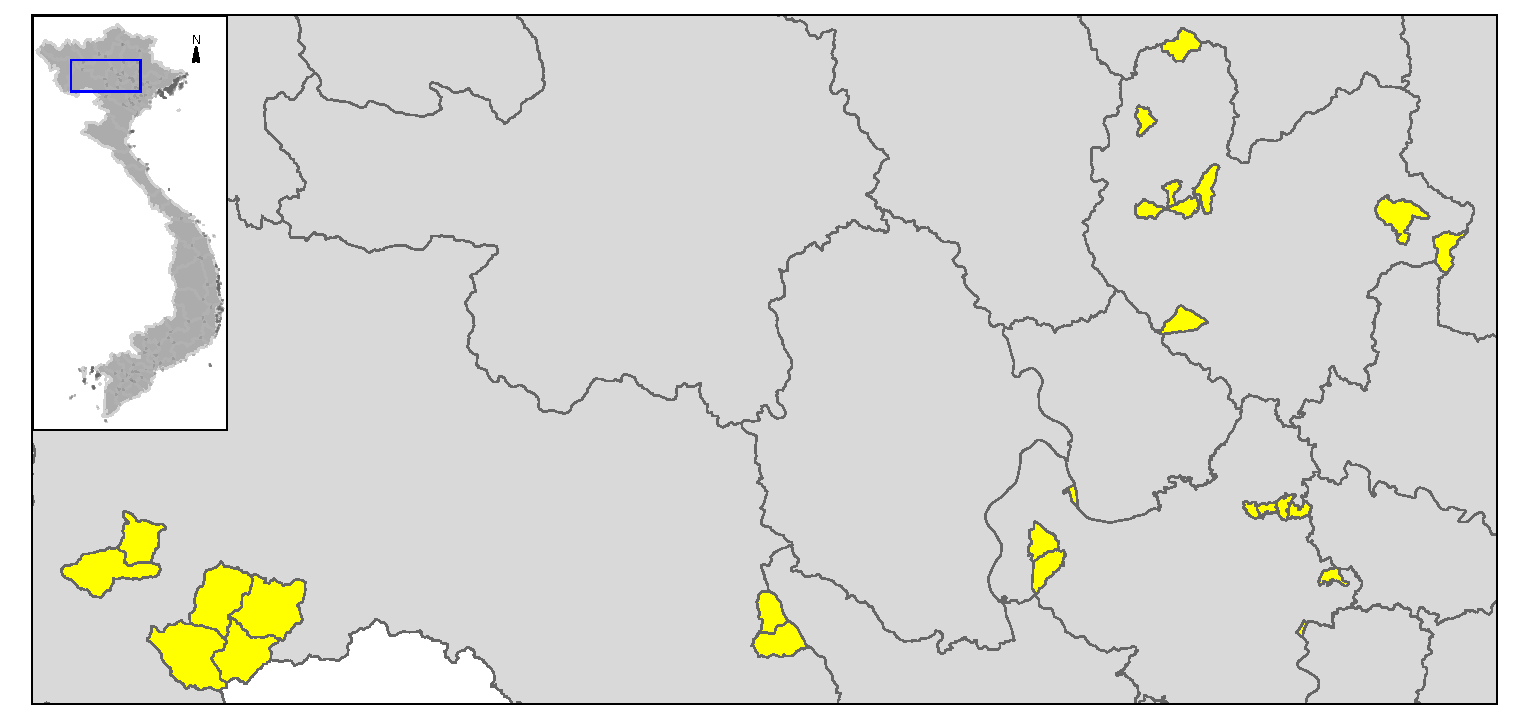
\includegraphics[width=1\textwidth]{map01.pdf}
\end{center}
\end{frame}

\begin{frame}
% latex table generated in R 4.2.1 by xtable 1.8-4 package
% Thu Oct 12 12:55:24 2023
\begin{table}[ht]
\centering
{\tiny%
\begin{tabular}{lrrrr}
  \toprule
Commune & summer & autumn & winter & spring \\
  \midrule
Bac Hong &   0 &   0 &   0 & 100 \\
  Binh Long &   0 &   0 & 100 &   0 \\
  Cat Ne &   0 & 100 &   0 &   0 \\
  Chieng Cang &   0 & 100 &   0 &   0 \\
  Chieng Khoong & 100 &   0 &   0 &   0 \\
  Chieng So &   0 &   0 &   0 &  85 \\
  Dong Dat &   0 &   0 &   0 &  99 \\
  Dong Thinh & 100 &   0 &   0 &   0 \\
  Duc Luong &   0 & 100 &   0 &   0 \\
  Hop Thanh &   0 &   0 &   0 & 101 \\
  Kim Lan &   0 & 100 &   0 &   0 \\
  Lien Hoa &   0 &   0 & 100 &   0 \\
  Linh Thong & 100 &   0 &   0 &   0 \\
  Minh Chau &  56 &   0 &   0 &   0 \\
  Muong Cai &   0 & 100 &   0 &   0 \\
  Muong Hung & 100 &   0 &   0 &   0 \\
  Nam Man &   0 &   0 &   0 & 115 \\
  Nguyen Khe &   0 &   0 &   0 & 100 \\
  Phu Dong &  82 &   0 &   0 &   0 \\
  Song Khua &   0 &   0 & 100 &   0 \\
  Tan Linh &  62 &  50 &   0 &   0 \\
  Thuy Lam &   0 &   0 & 100 &   0 \\
  Trang &   0 &   0 & 100 &   0 \\
  Van Hoa &   0 &  50 &   0 &   0 \\
  Xuan Non &   0 &   0 & 100 &   0 \\
   \bottomrule
\end{tabular}}
\end{table}
\end{frame}


\begin{frame}
\begin{center}
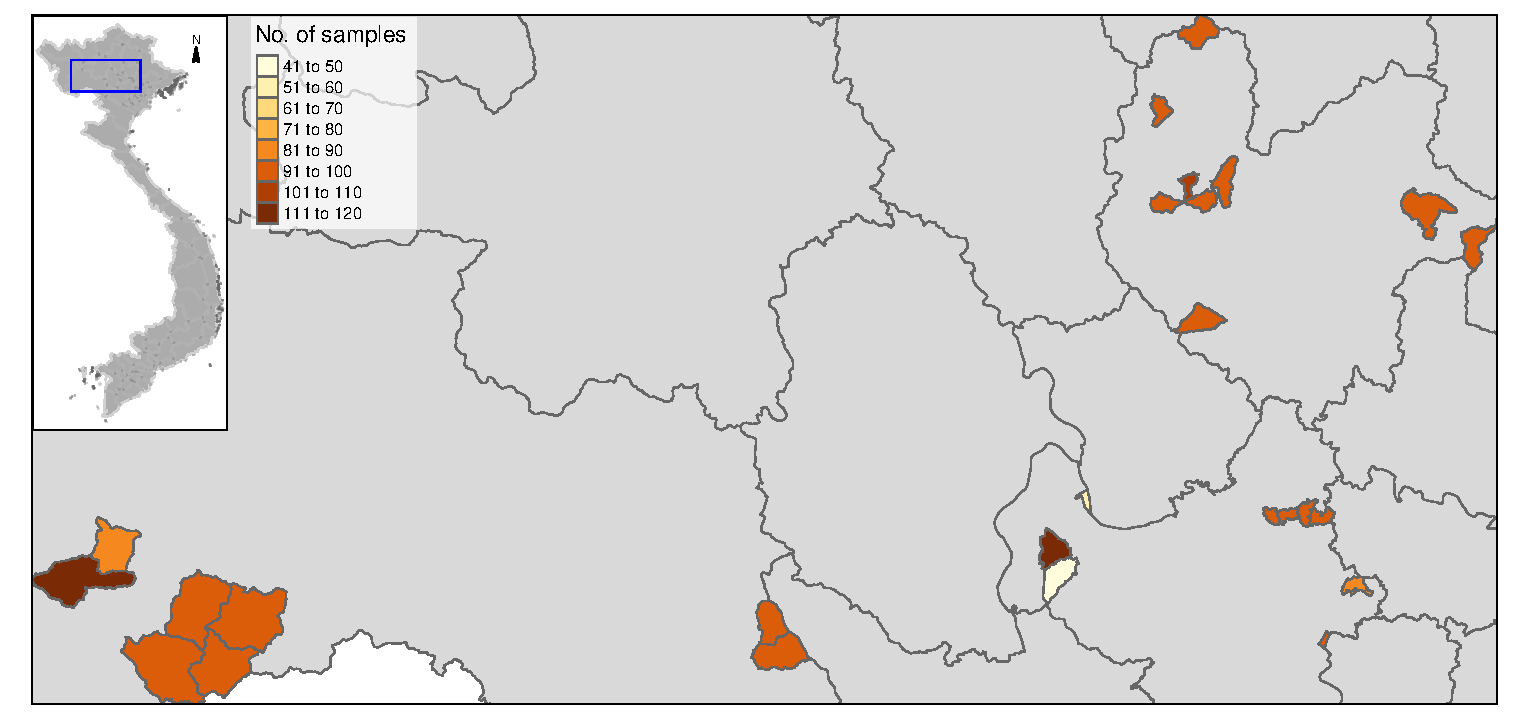
\includegraphics[width=1\textwidth]{map02.pdf}
\end{center}
\end{frame}

\begin{frame}
summer\\
\begin{center}
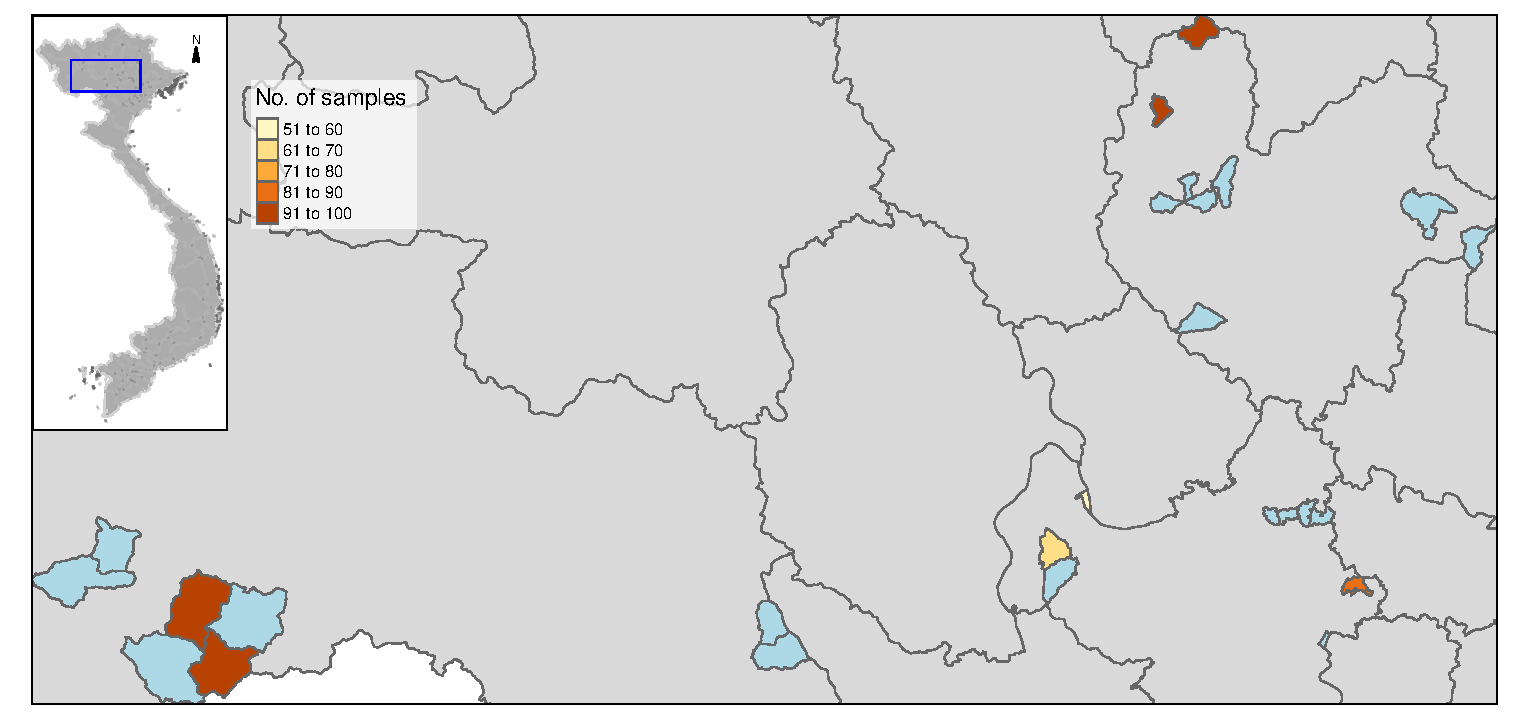
\includegraphics[width=1\textwidth]{map02_summer.pdf}
\end{center}
\end{frame}


\begin{frame}
autumn\\
\begin{center}
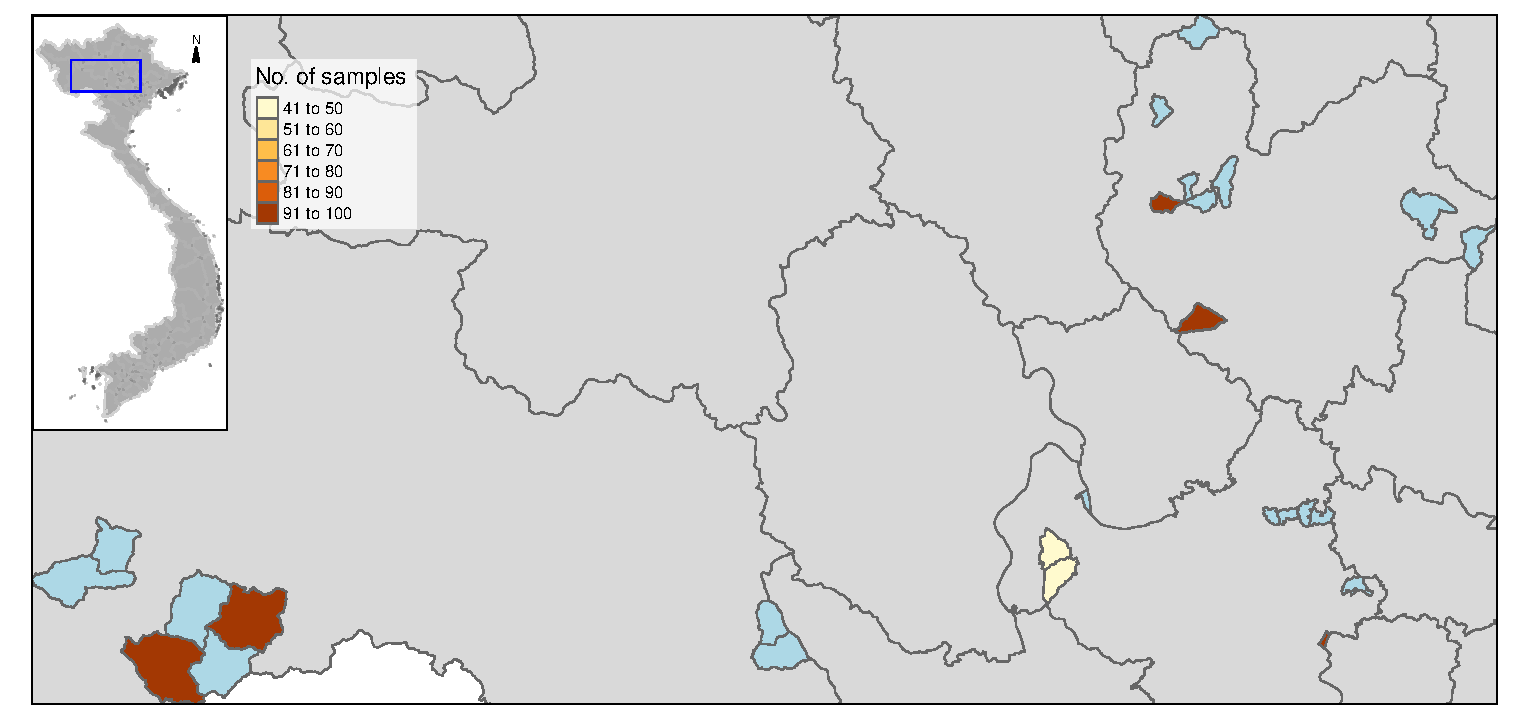
\includegraphics[width=1\textwidth]{map02_autumn.pdf}
\end{center}
\end{frame}

\begin{frame}
winter\\
\begin{center}
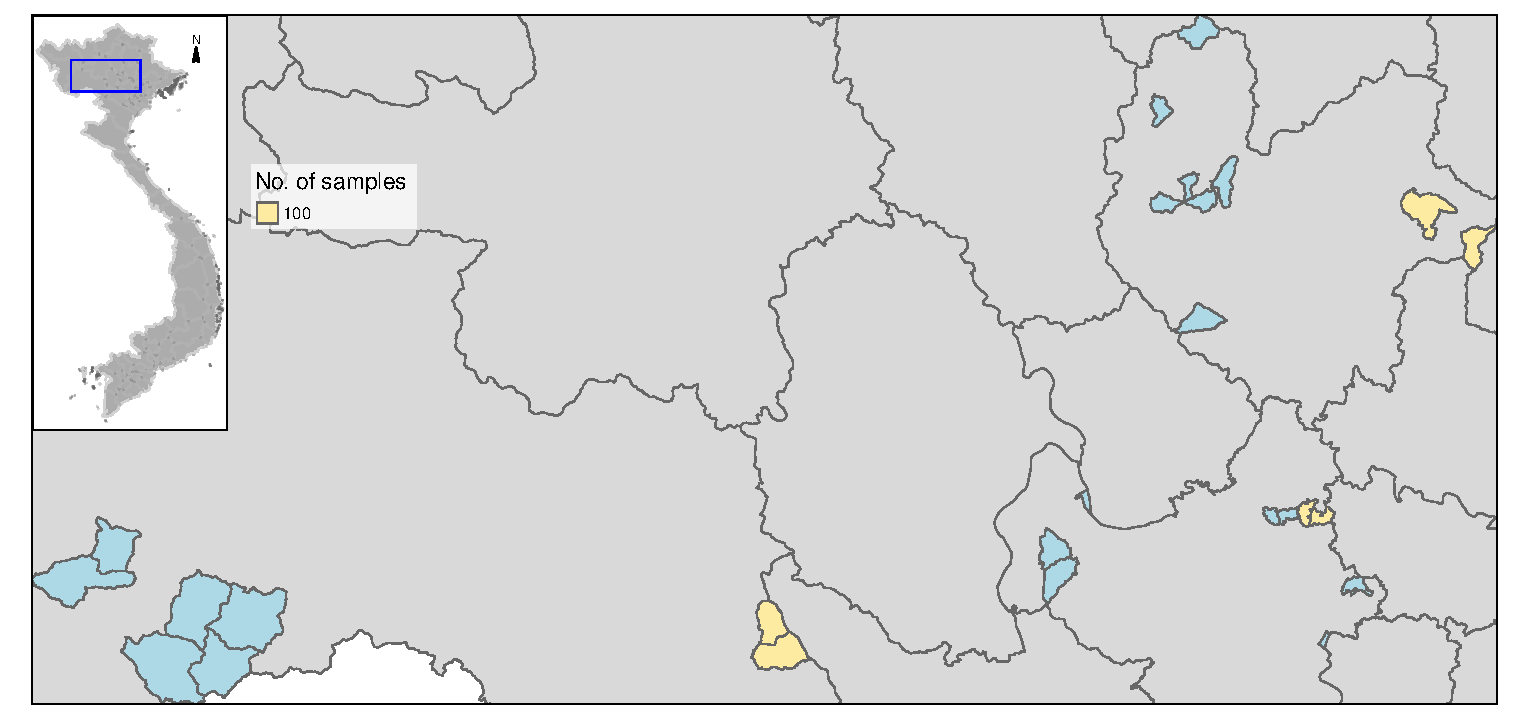
\includegraphics[width=1\textwidth]{map02_winter.pdf}
\end{center}
\end{frame}


\begin{frame}
spring\\
\begin{center}
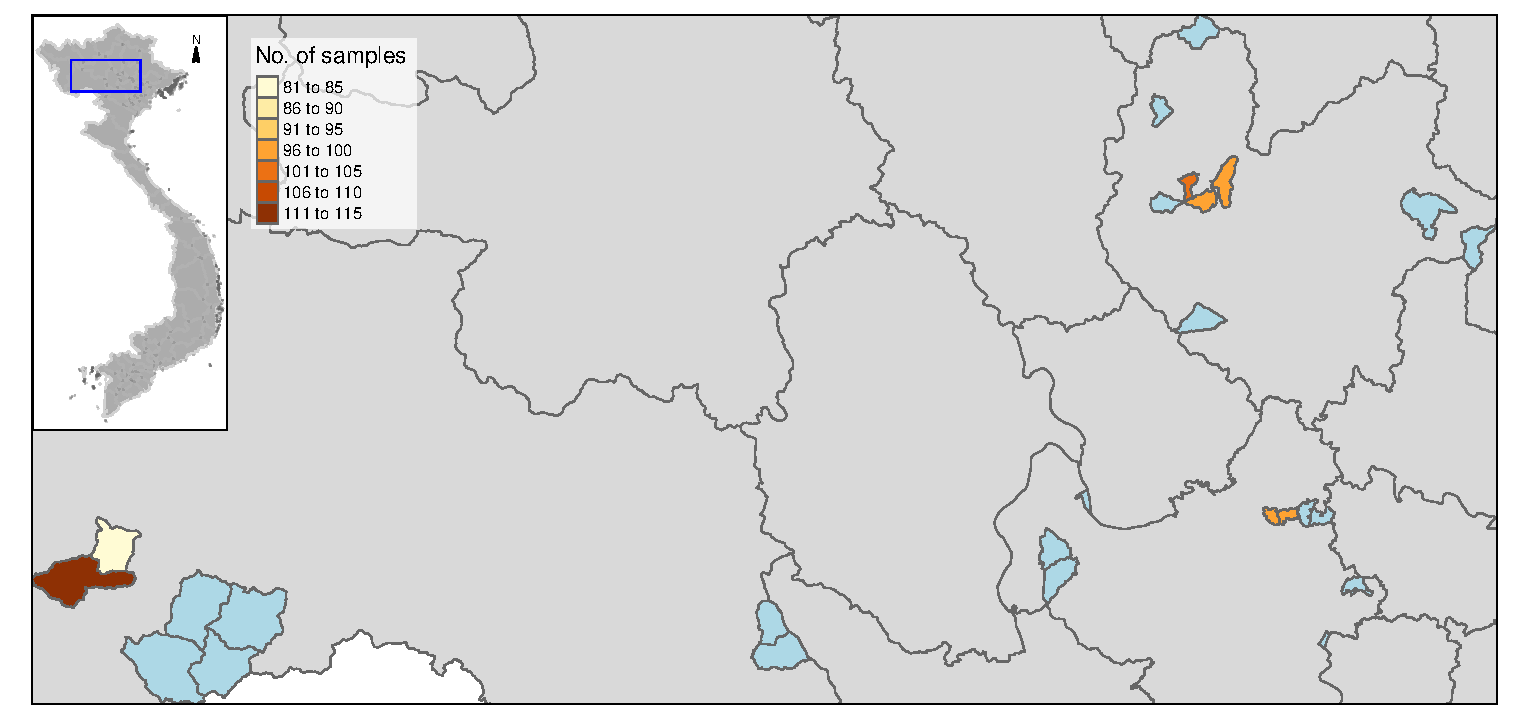
\includegraphics[width=1\textwidth]{map02_spring.pdf}
\end{center}
\end{frame}

\section{Prevalence}
\begin{frame}
\begin{center}
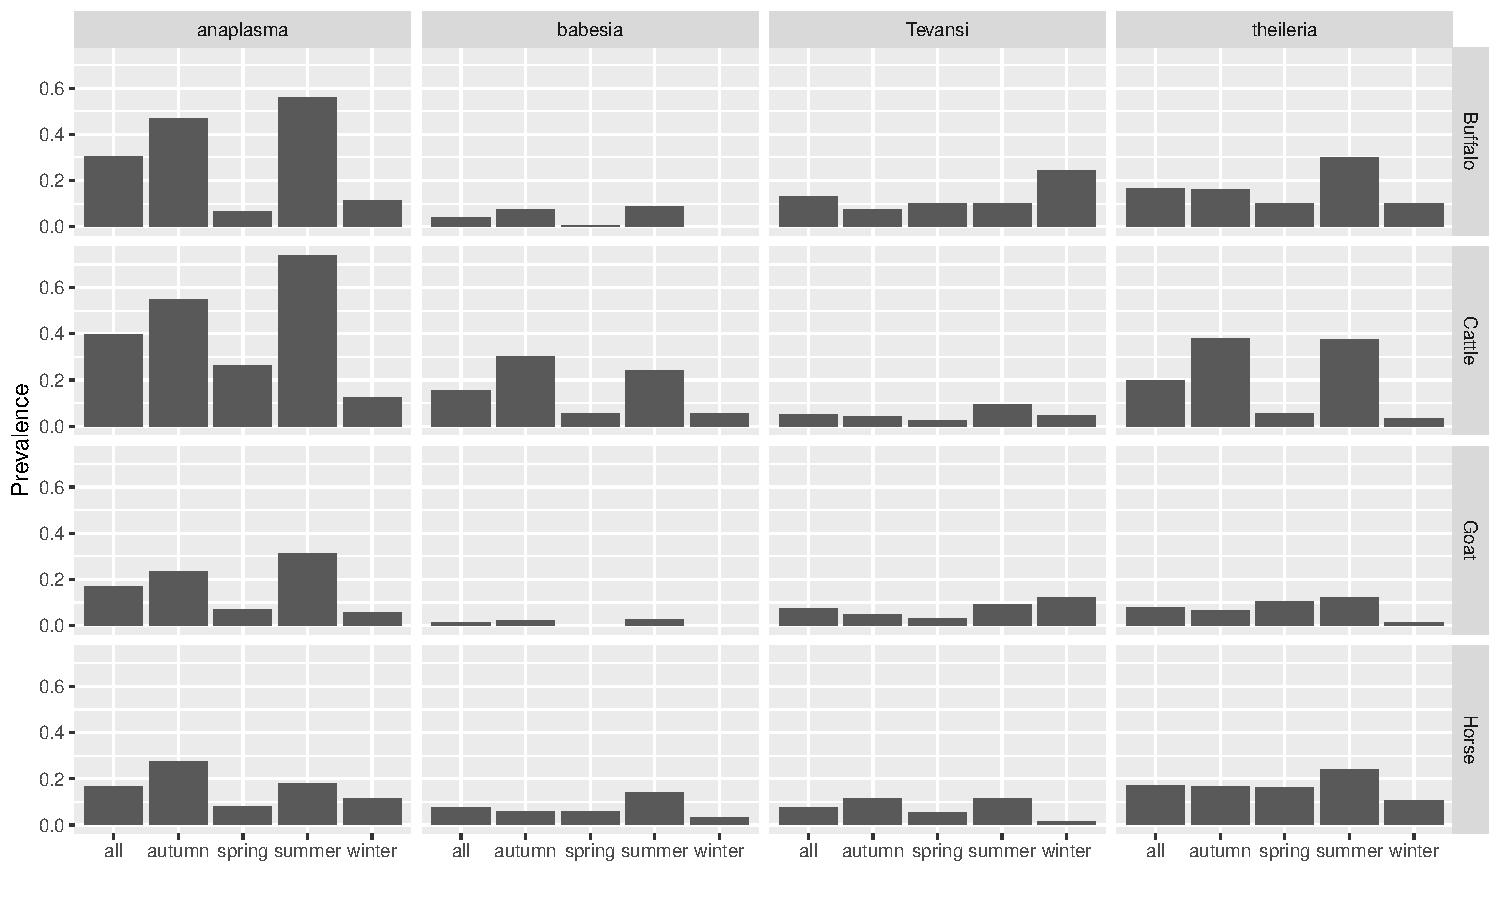
\includegraphics[width=1\textwidth]{fig_prev01.pdf}
\end{center}
\end{frame}


\subsection{Anaplasma}
\begin{frame}
\begin{center}
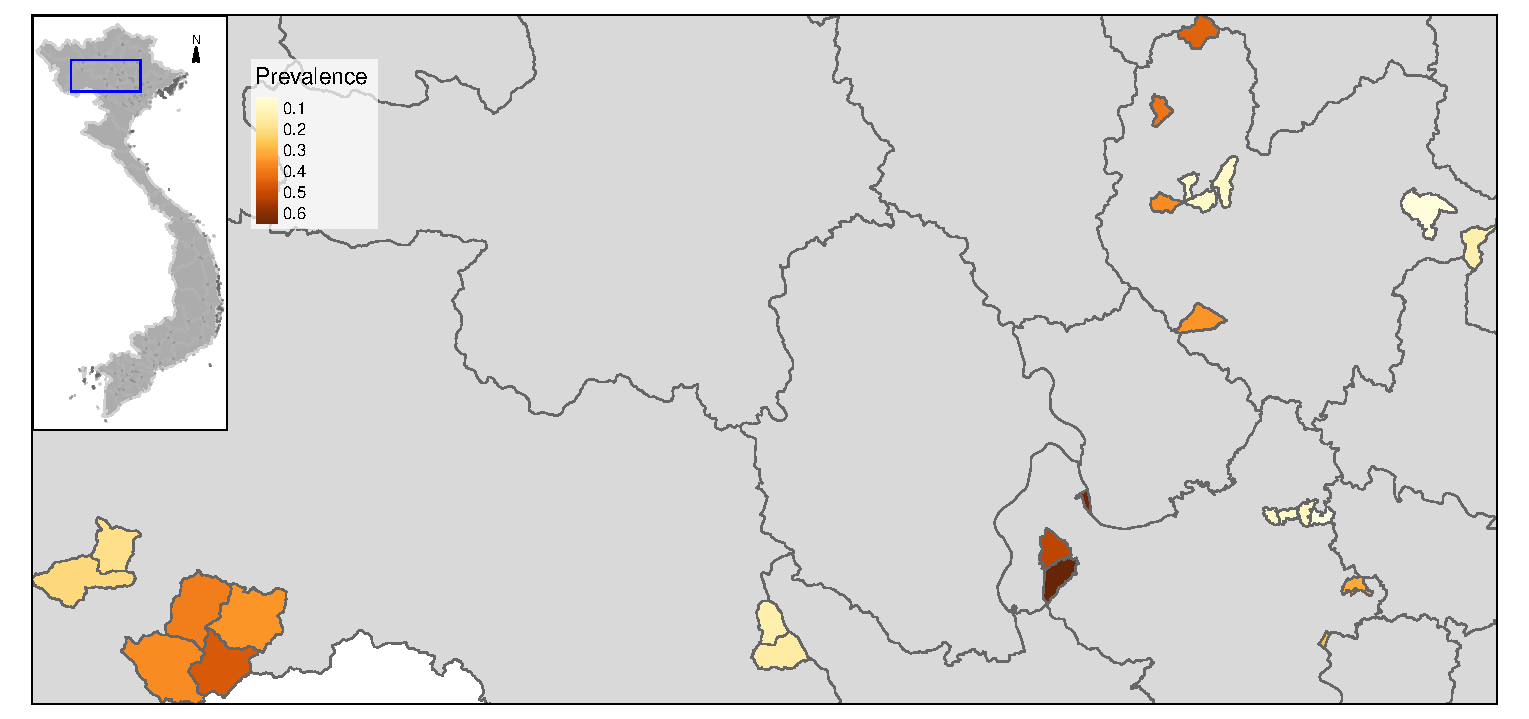
\includegraphics[width=1\textwidth]{map03.pdf}
\end{center}
\end{frame}

\begin{frame}
summer\\
\begin{center}
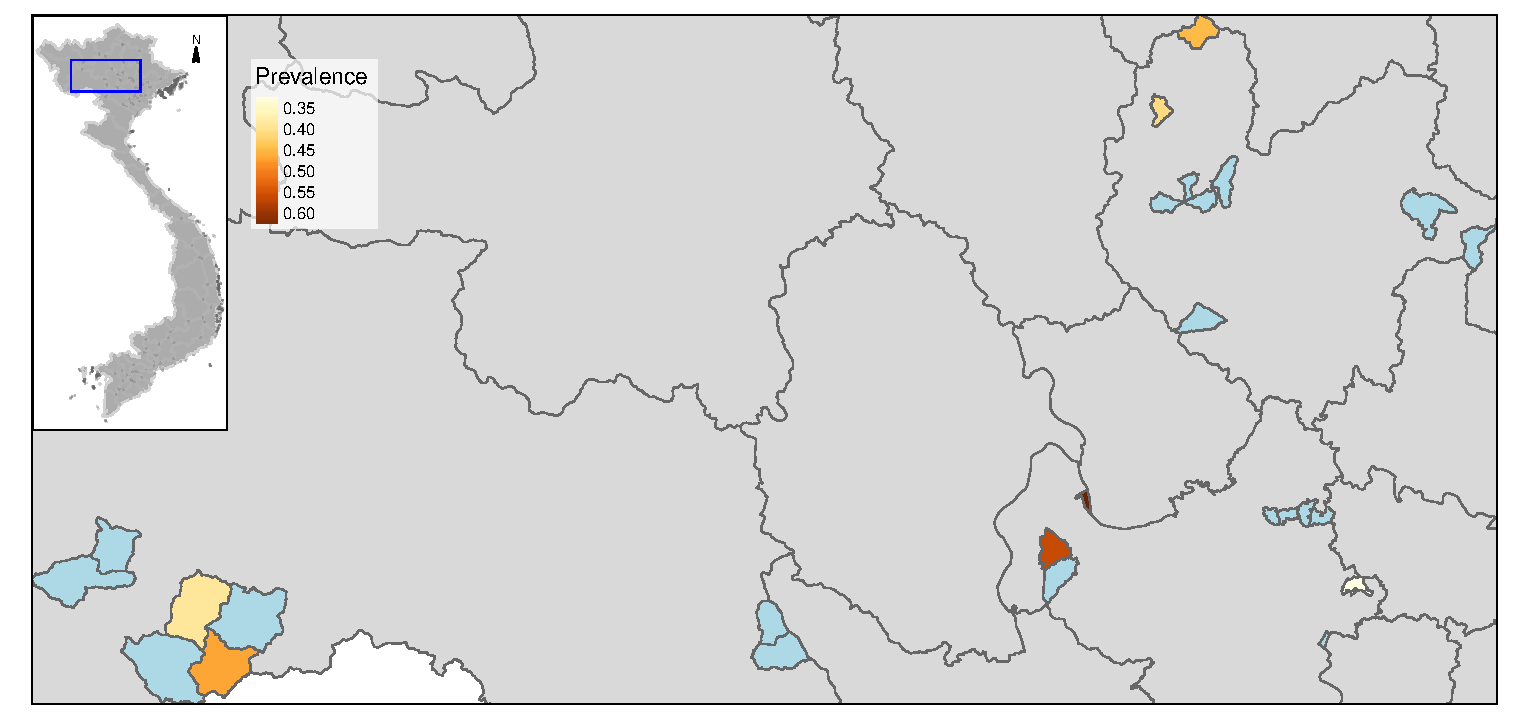
\includegraphics[width=1\textwidth]{map03_summer.pdf}
\end{center}
\end{frame}


\begin{frame}
autumn\\
\begin{center}
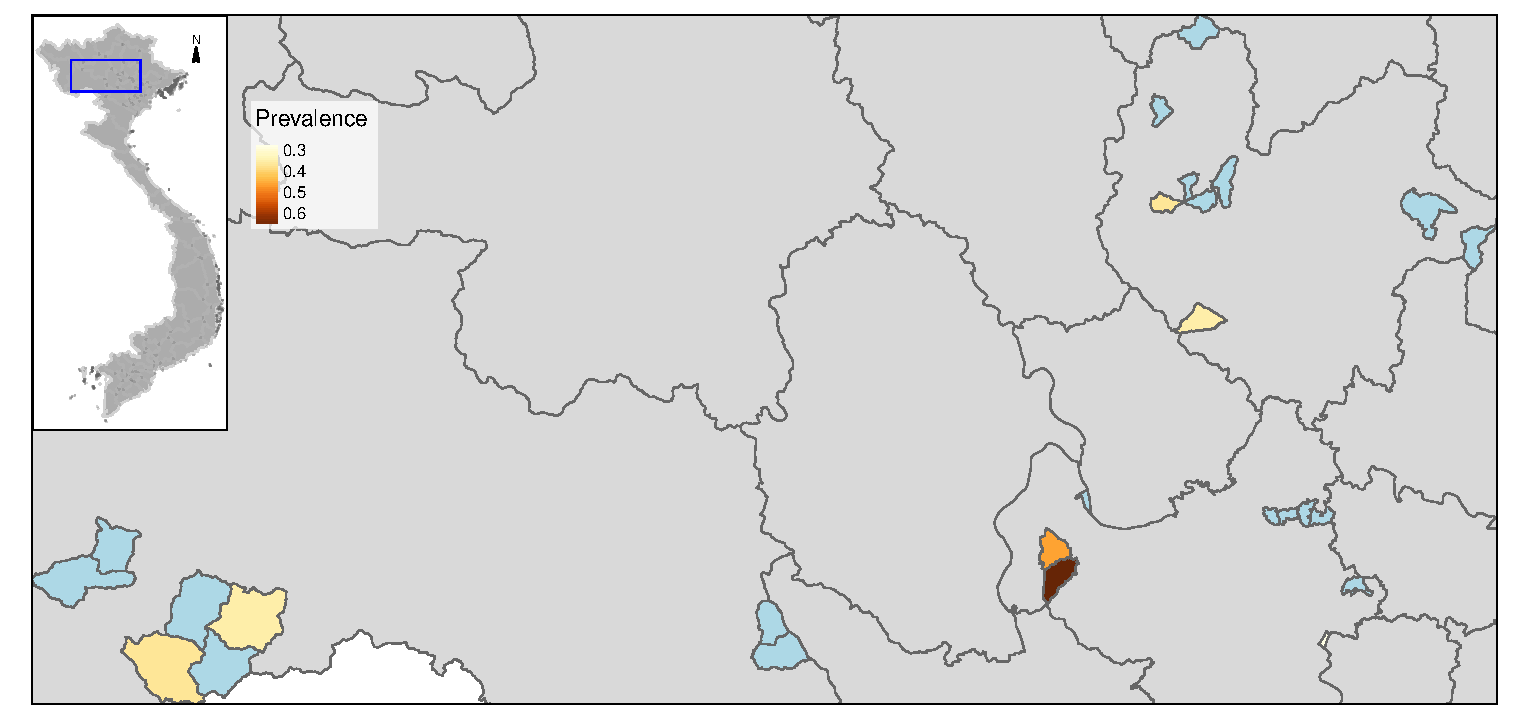
\includegraphics[width=1\textwidth]{map03_autumn.pdf}
\end{center}
\end{frame}

\begin{frame}
winter\\
\begin{center}
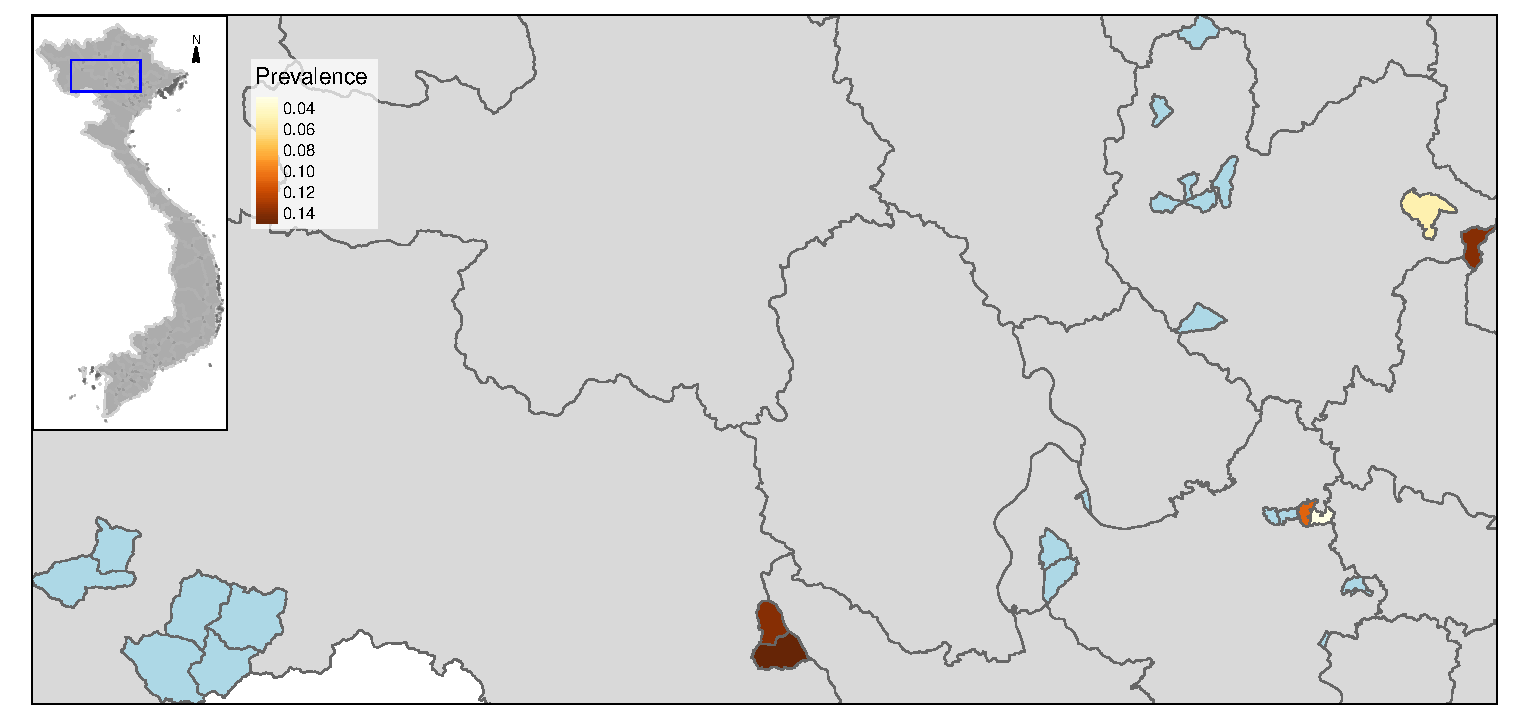
\includegraphics[width=1\textwidth]{map03_winter.pdf}
\end{center}
\end{frame}


\begin{frame}
spring\\
\begin{center}
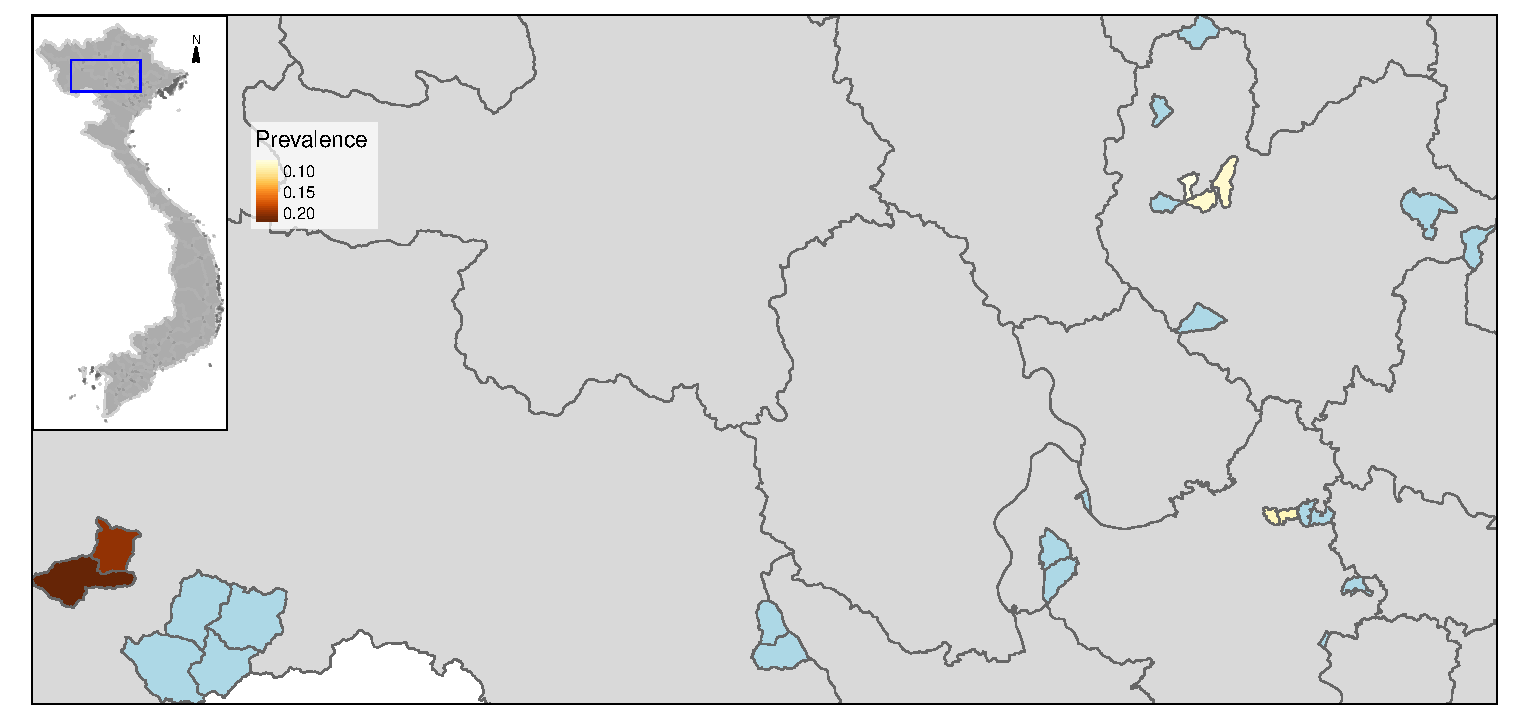
\includegraphics[width=1\textwidth]{map03_spring.pdf}
\end{center}
\end{frame}

\subsection{Babesia}
\begin{frame}
\begin{center}
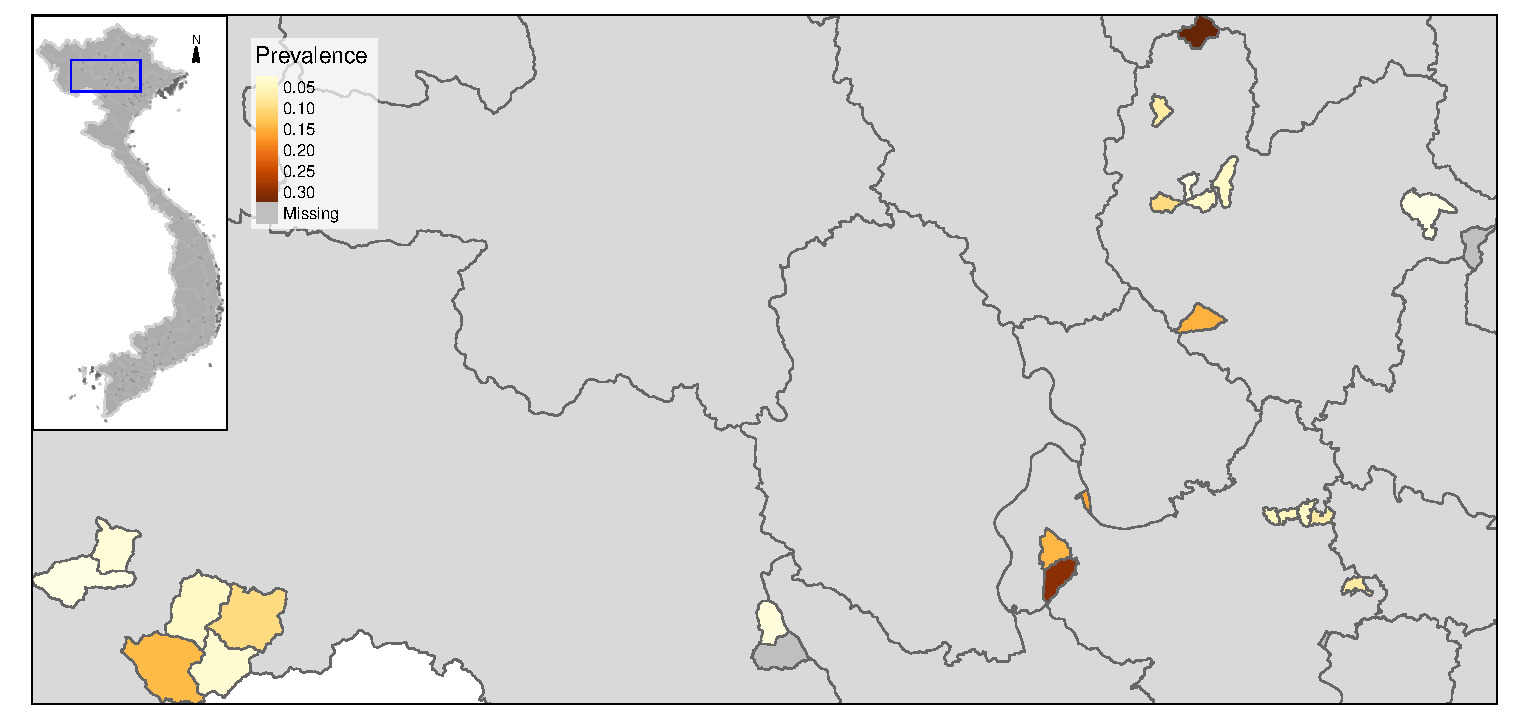
\includegraphics[width=1\textwidth]{map04.pdf}
\end{center}
\end{frame}

\begin{frame}
summer\\
\begin{center}
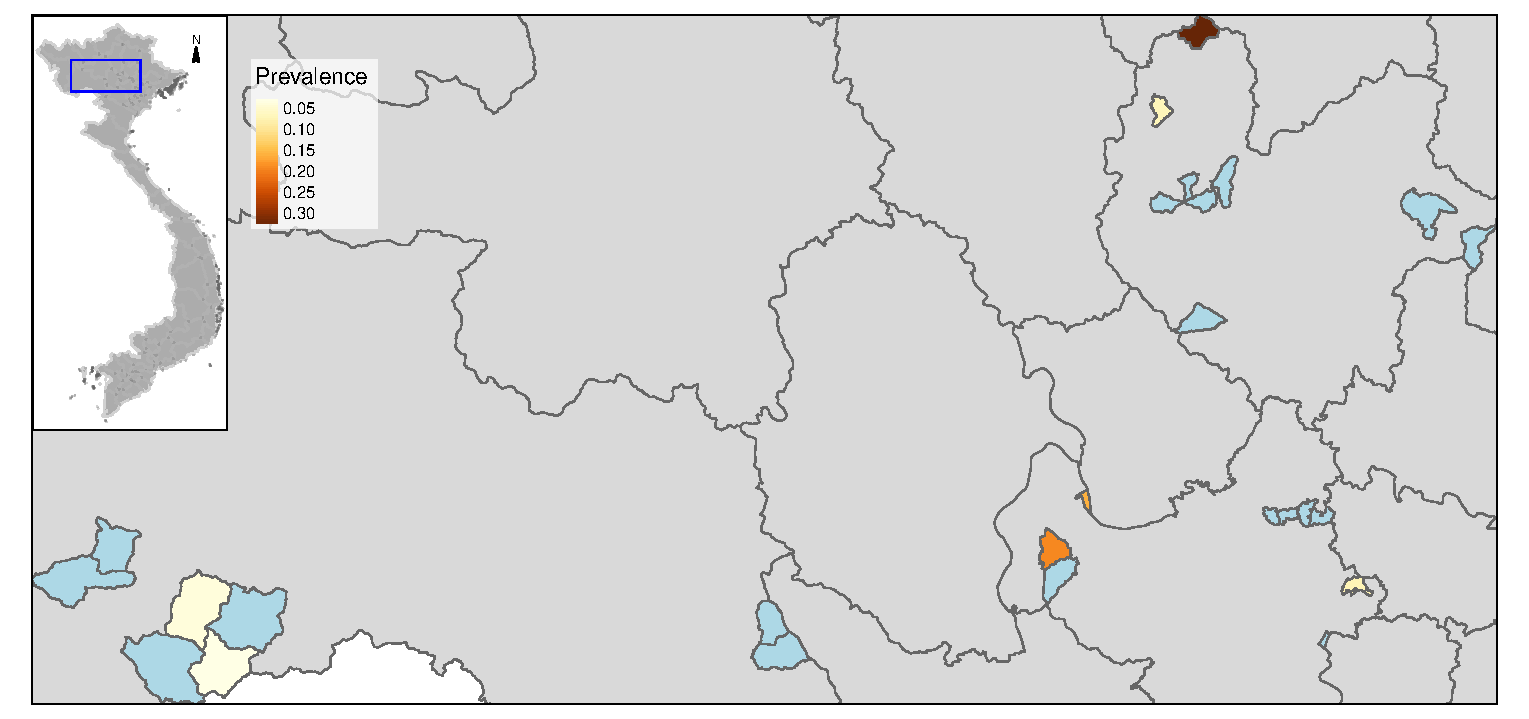
\includegraphics[width=1\textwidth]{map04_summer.pdf}
\end{center}
\end{frame}


\begin{frame}
autumn\\
\begin{center}
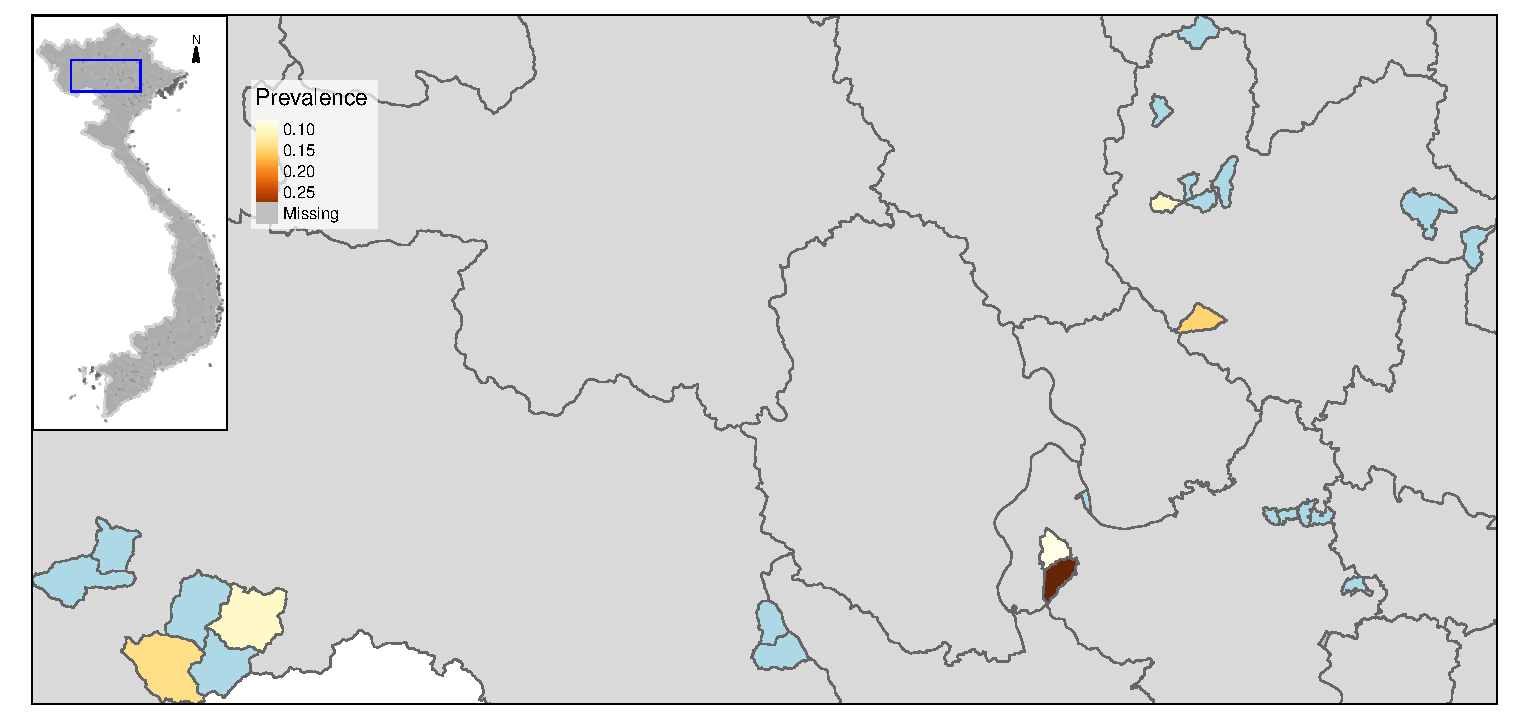
\includegraphics[width=1\textwidth]{map04_autumn.pdf}
\end{center}
\end{frame}

\begin{frame}
winter\\
\begin{center}
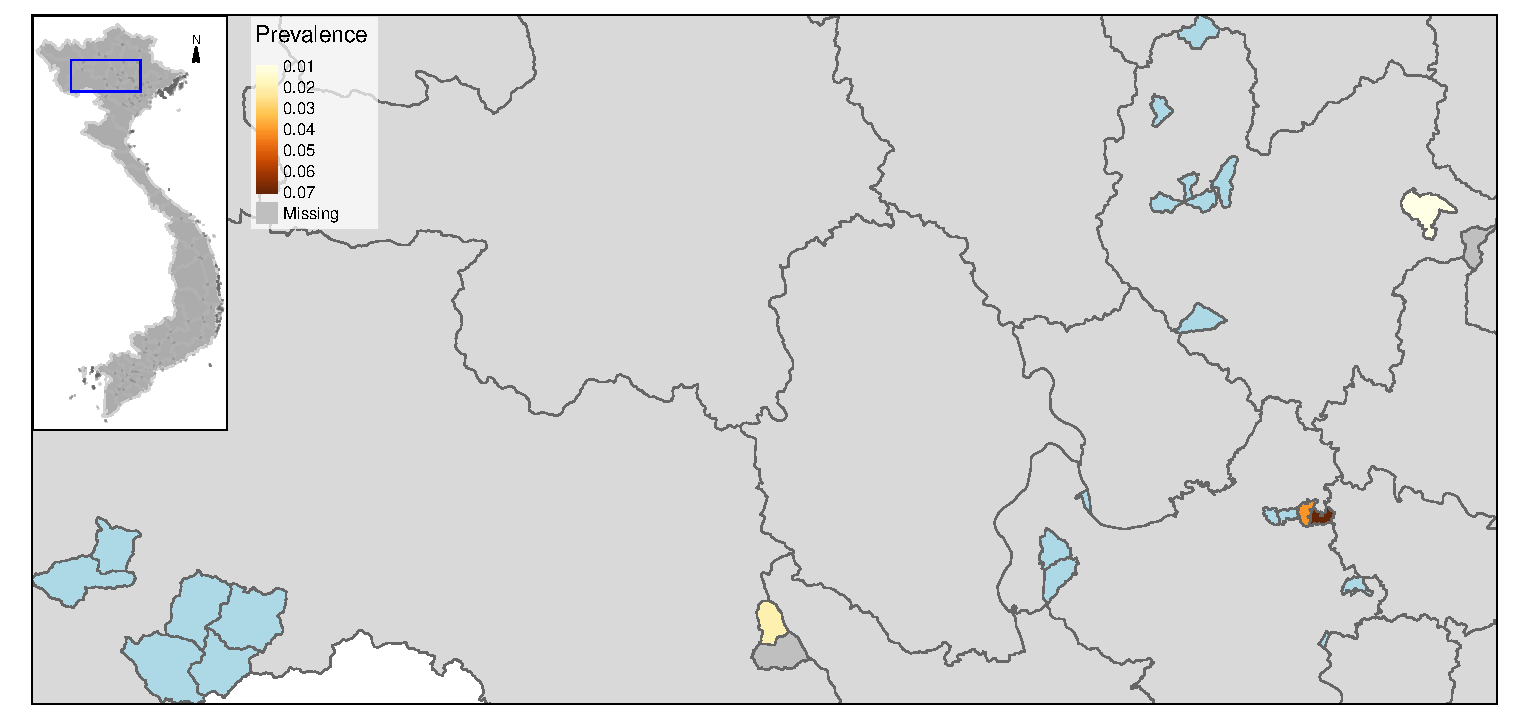
\includegraphics[width=1\textwidth]{map04_winter.pdf}
\end{center}
\end{frame}


\begin{frame}
spring\\
\begin{center}
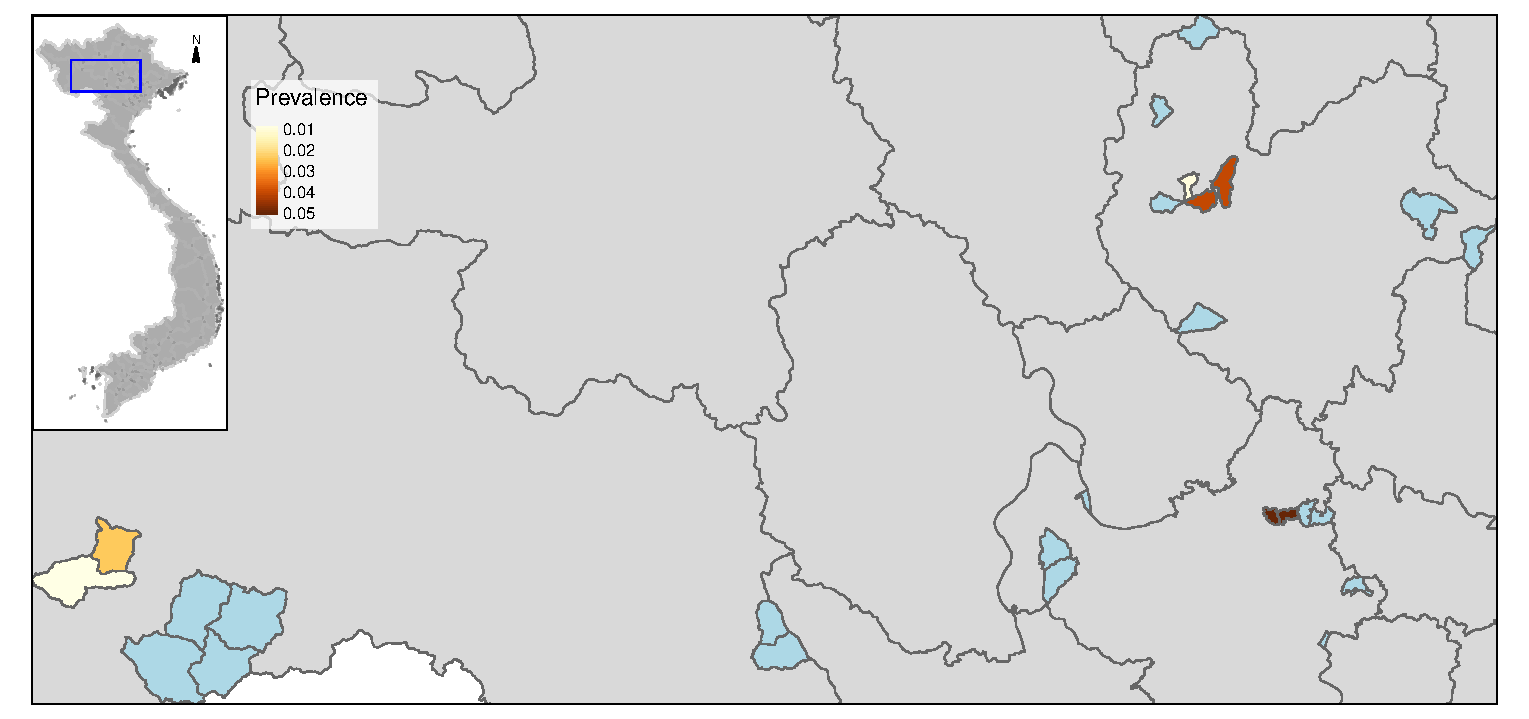
\includegraphics[width=1\textwidth]{map04_spring.pdf}
\end{center}
\end{frame}


\subsection{Theileria}
\begin{frame}
\begin{center}
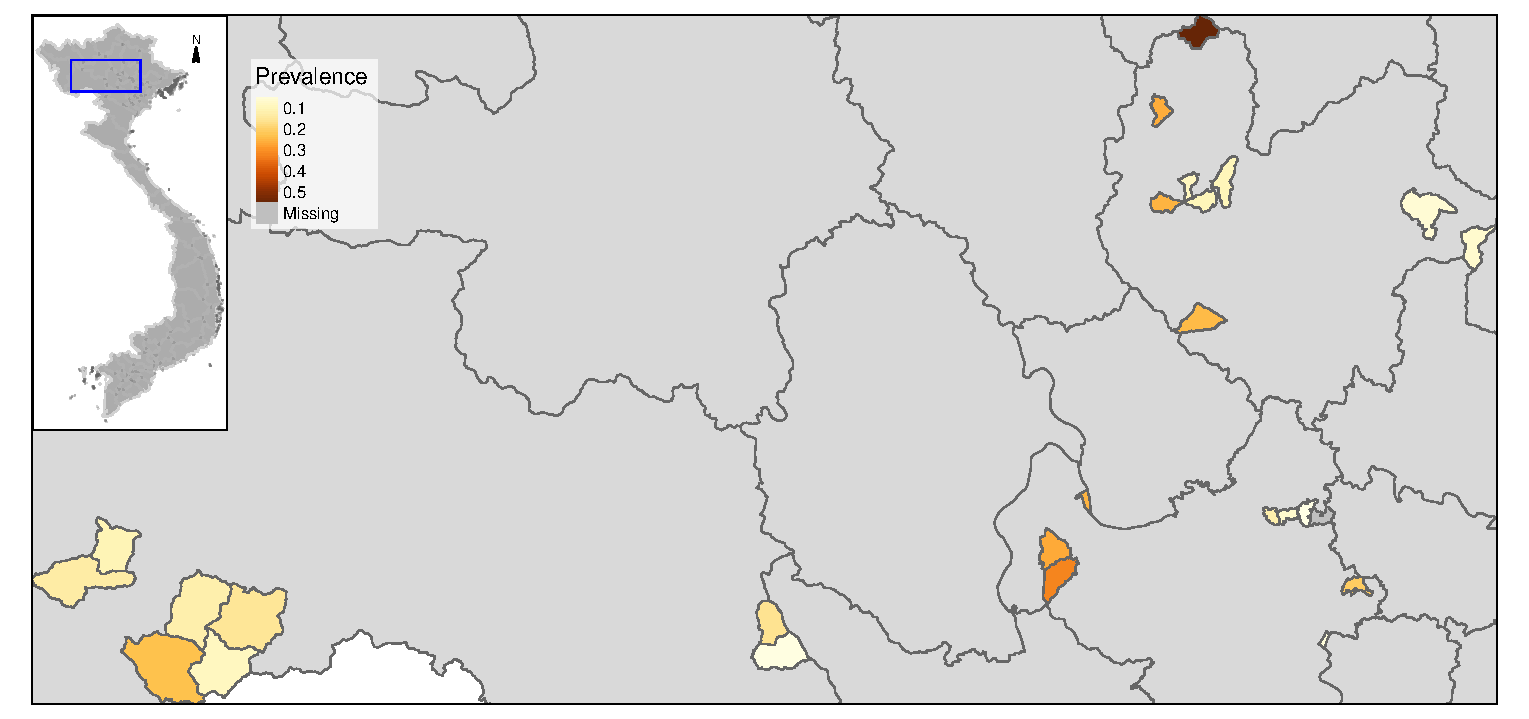
\includegraphics[width=1\textwidth]{map05.pdf}
\end{center}
\end{frame}

\begin{frame}
summer\\
\begin{center}
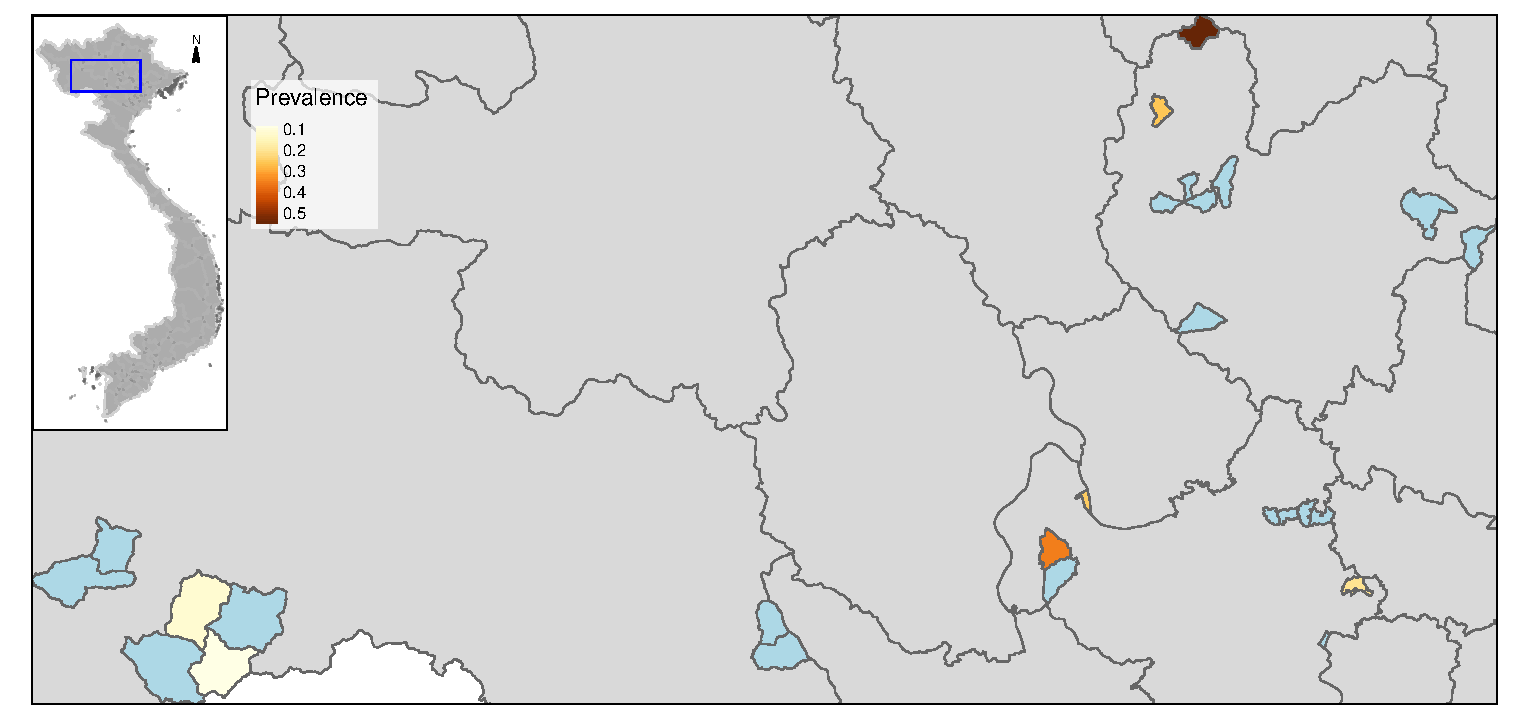
\includegraphics[width=1\textwidth]{map05_summer.pdf}
\end{center}
\end{frame}


\begin{frame}
autumn\\
\begin{center}
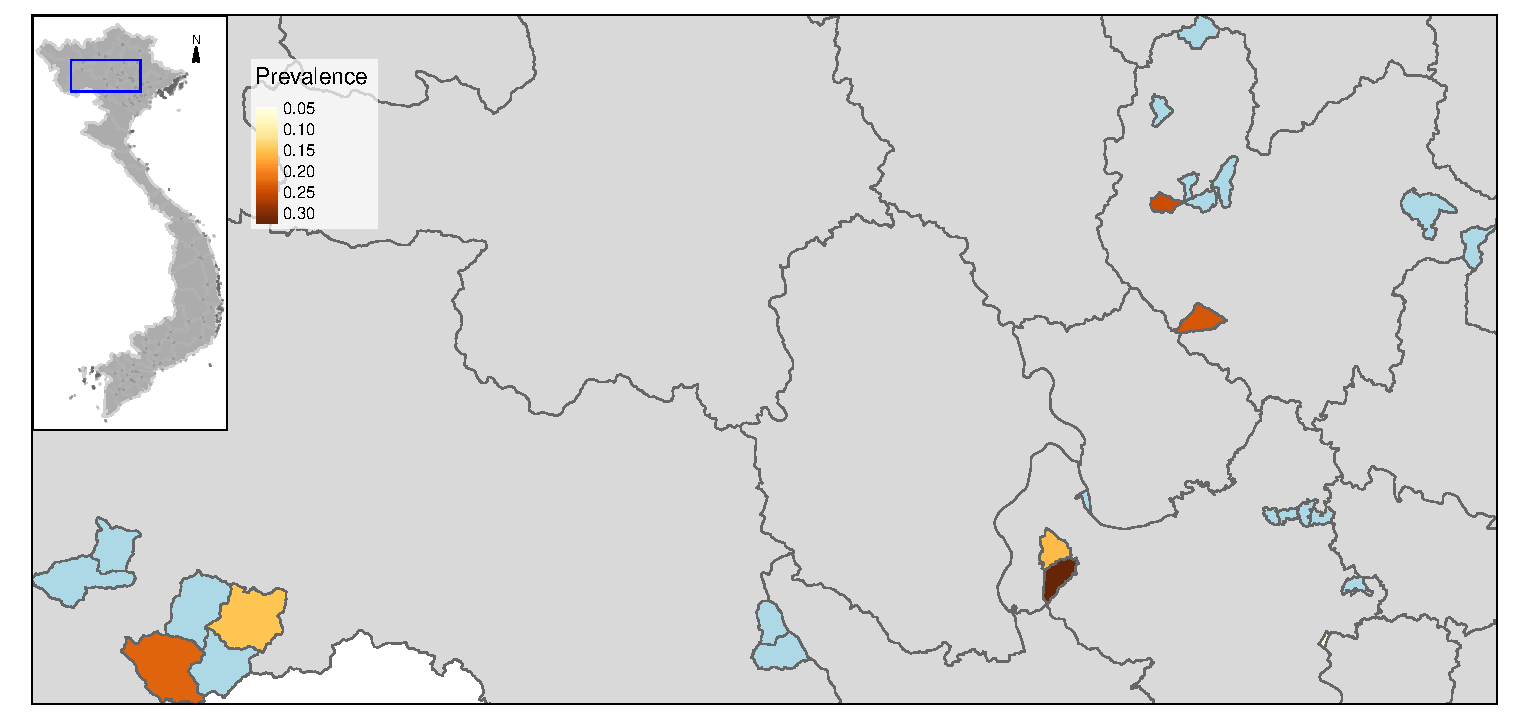
\includegraphics[width=1\textwidth]{map05_autumn.pdf}
\end{center}
\end{frame}

\begin{frame}
winter\\
\begin{center}
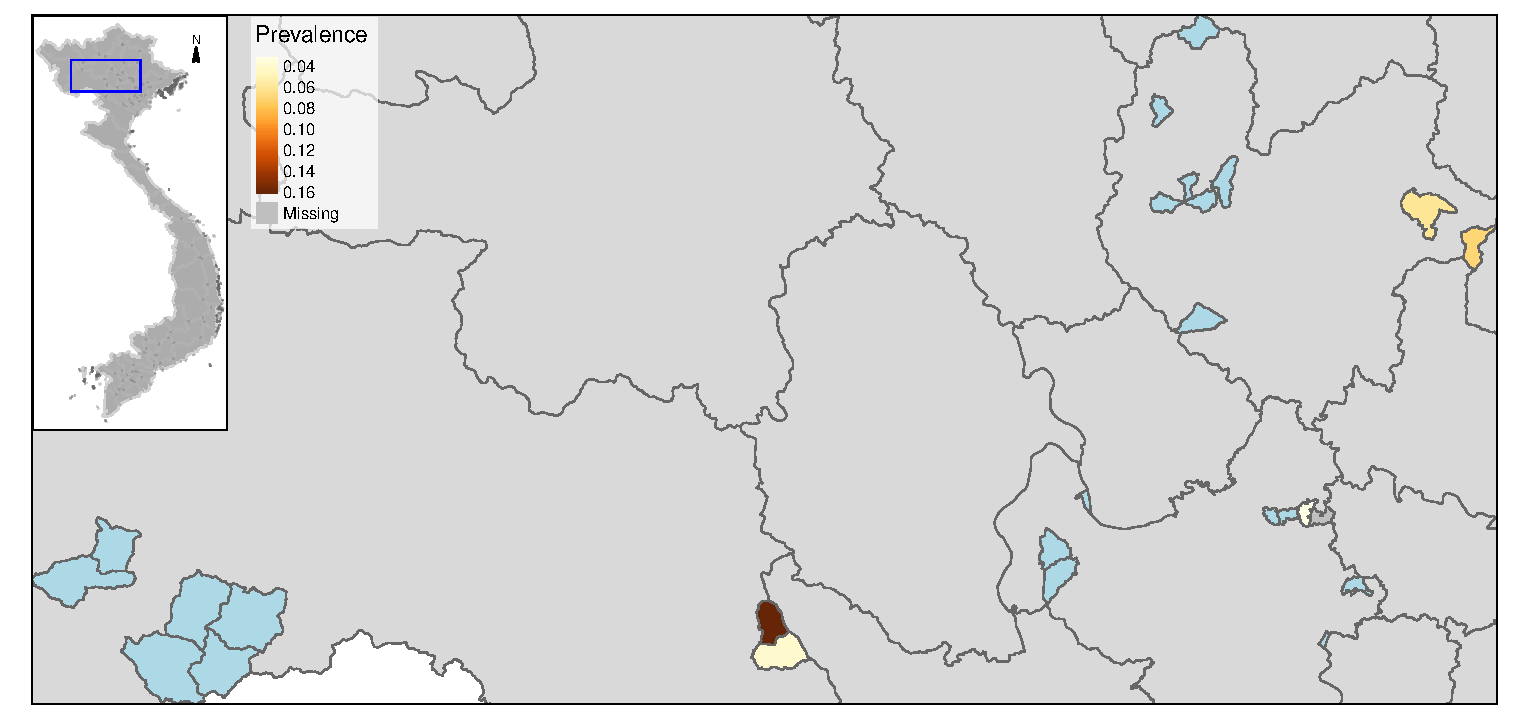
\includegraphics[width=1\textwidth]{map05_winter.pdf}
\end{center}
\end{frame}


\begin{frame}
spring\\
\begin{center}
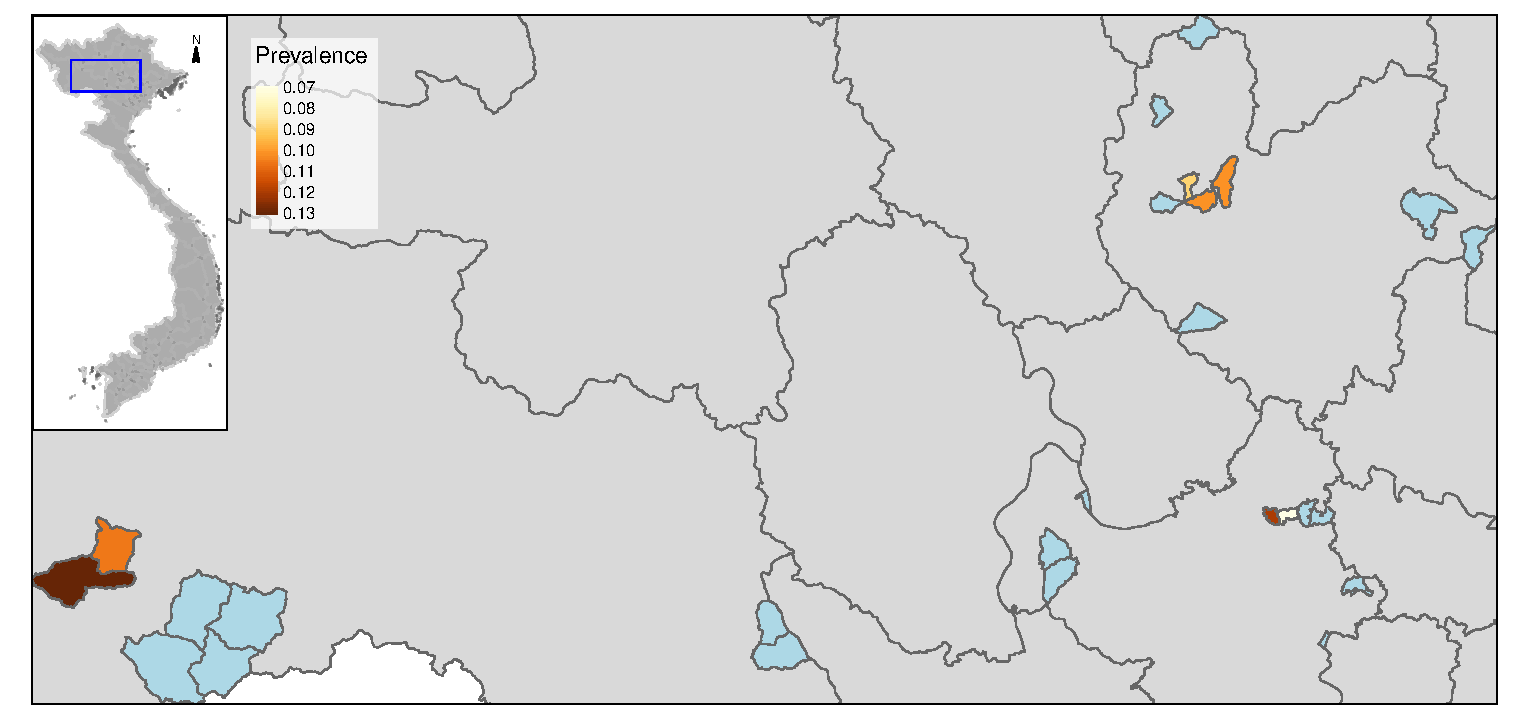
\includegraphics[width=1\textwidth]{map05_spring.pdf}
\end{center}
\end{frame}


\subsection{\textit{Trypanosoma evansi}}
\begin{frame}
\begin{center}
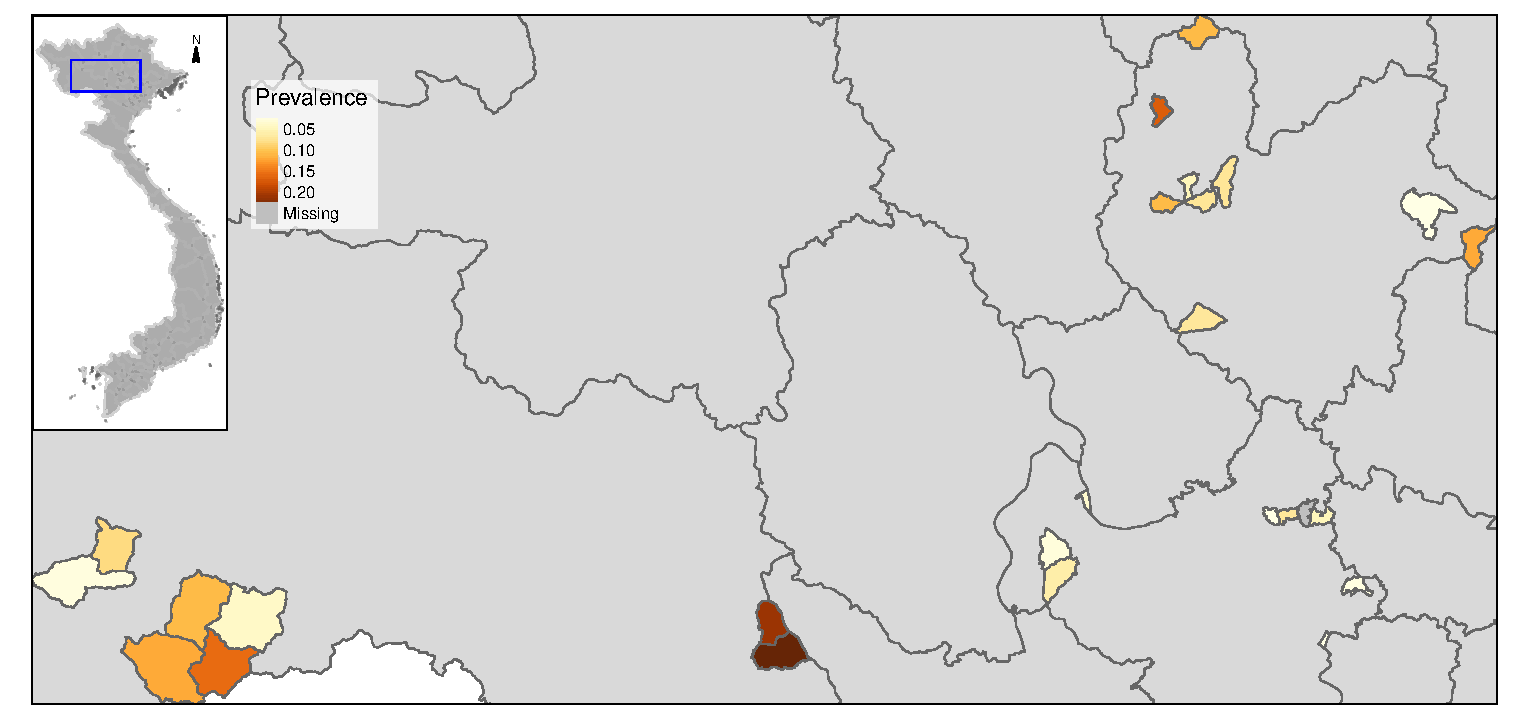
\includegraphics[width=1\textwidth]{map06.pdf}
\end{center}
\end{frame}

\begin{frame}
summer\\
\begin{center}
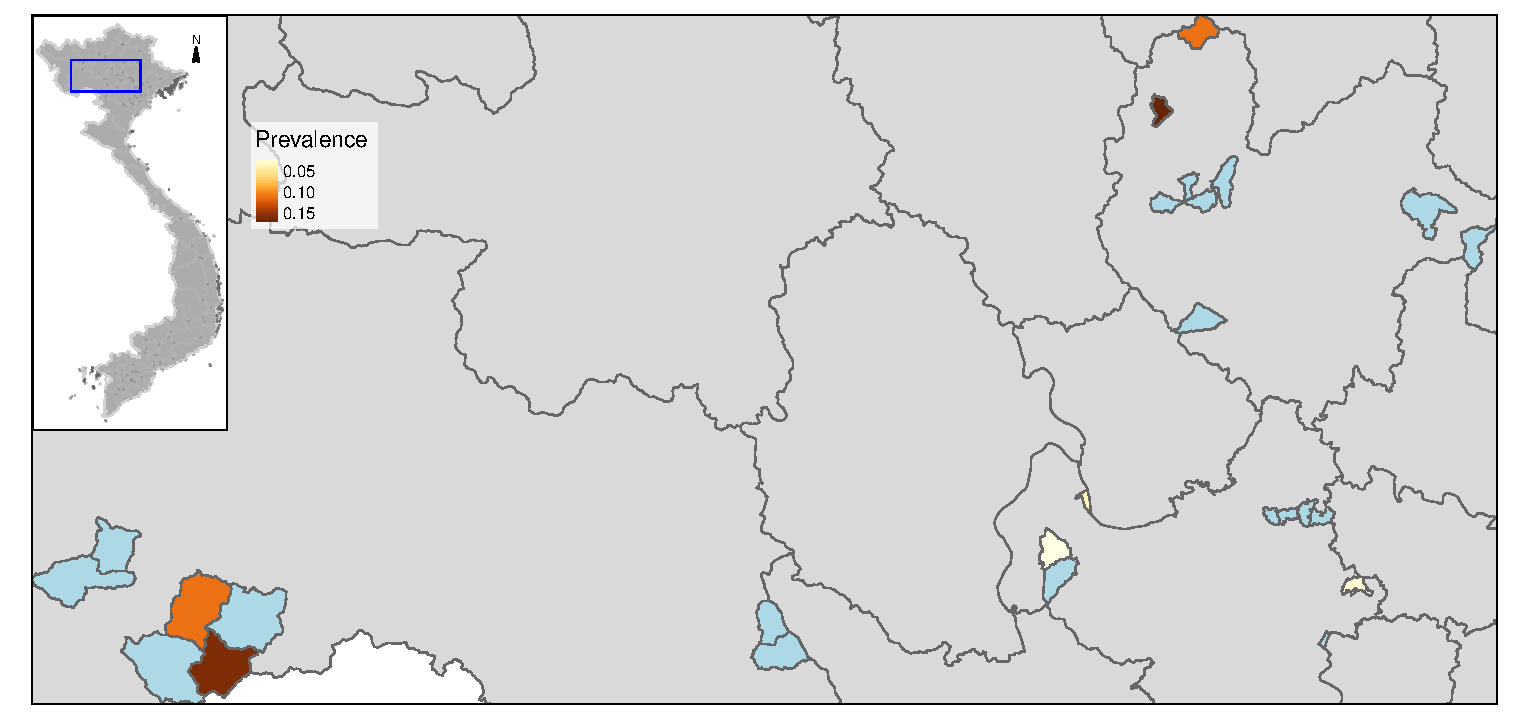
\includegraphics[width=1\textwidth]{map06_summer.pdf}
\end{center}
\end{frame}


\begin{frame}
autumn\\
\begin{center}
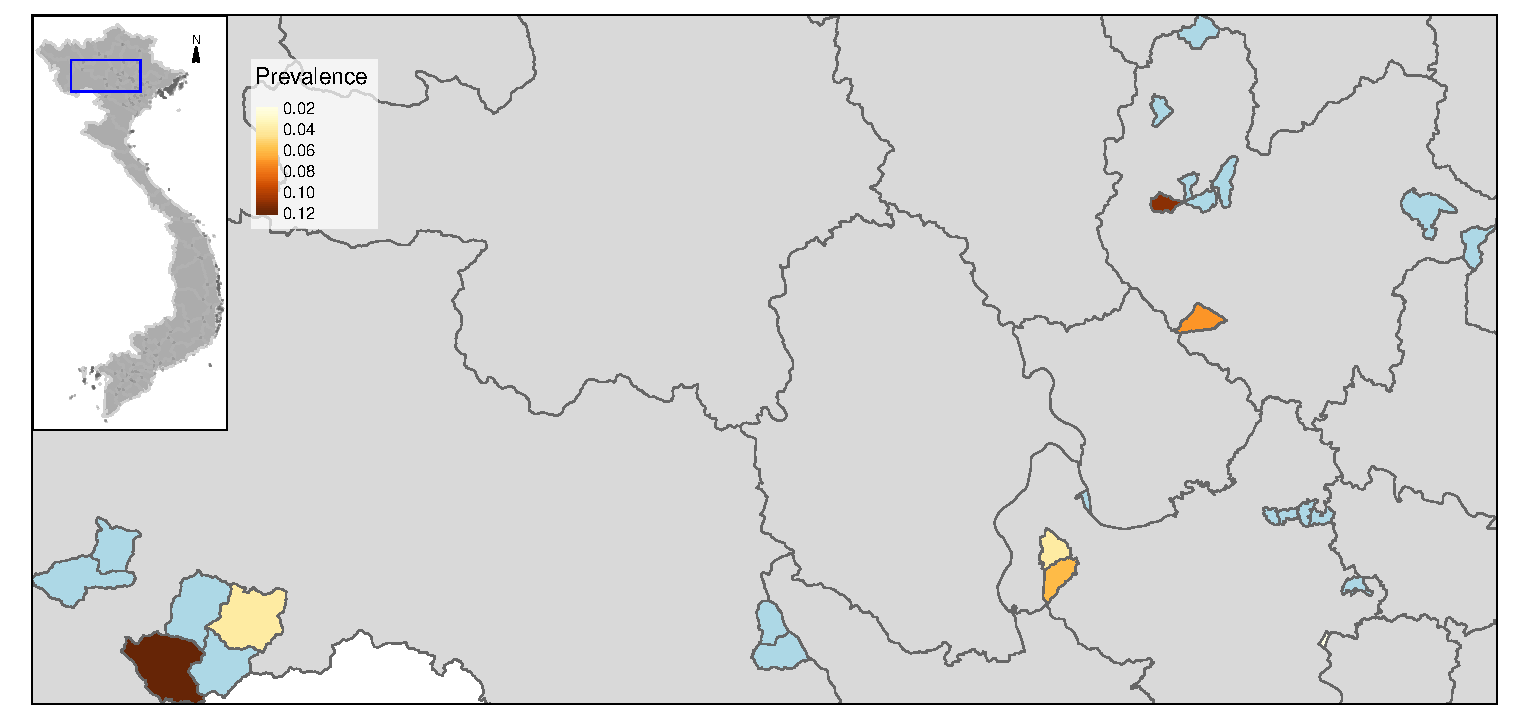
\includegraphics[width=1\textwidth]{map06_autumn.pdf}
\end{center}
\end{frame}

\begin{frame}
winter\\
\begin{center}
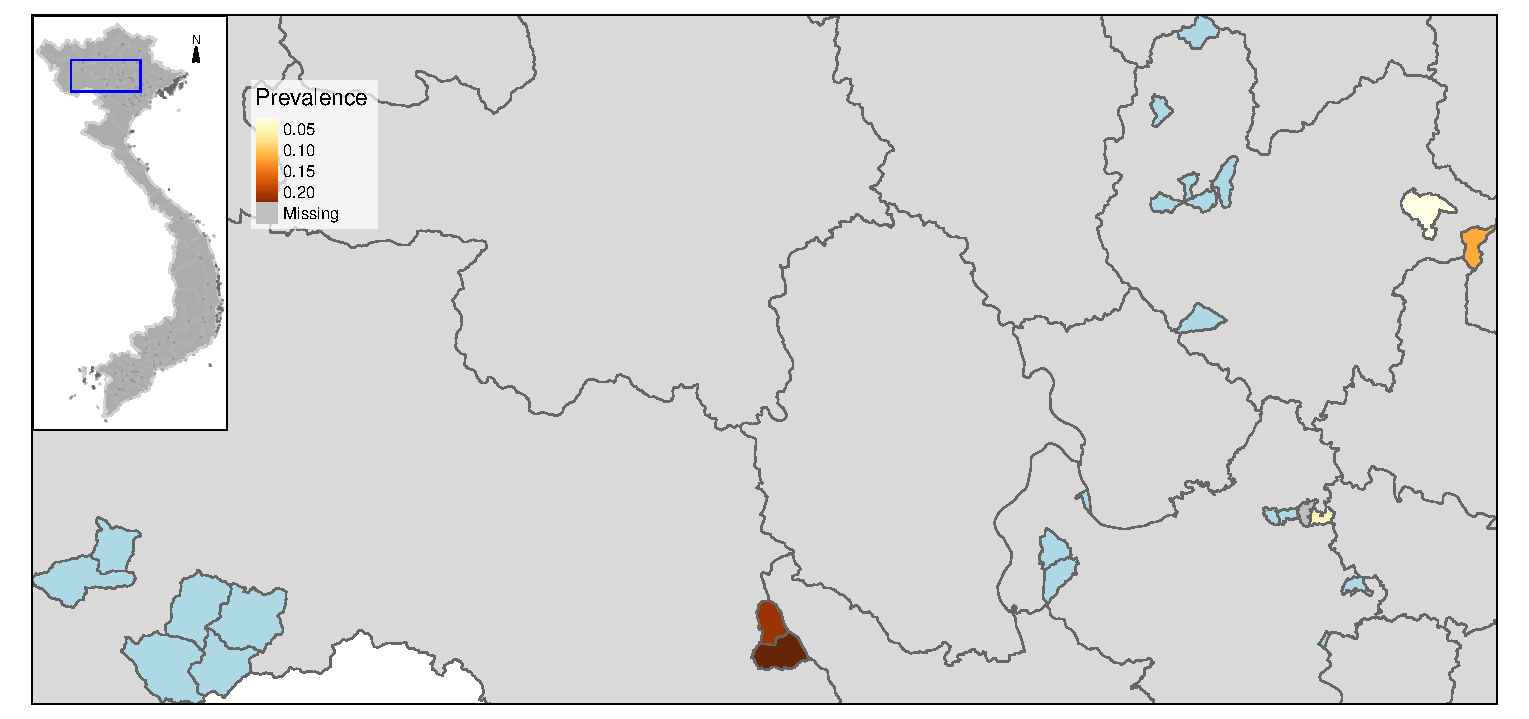
\includegraphics[width=1\textwidth]{map06_winter.pdf}
\end{center}
\end{frame}


\begin{frame}
spring\\
\begin{center}
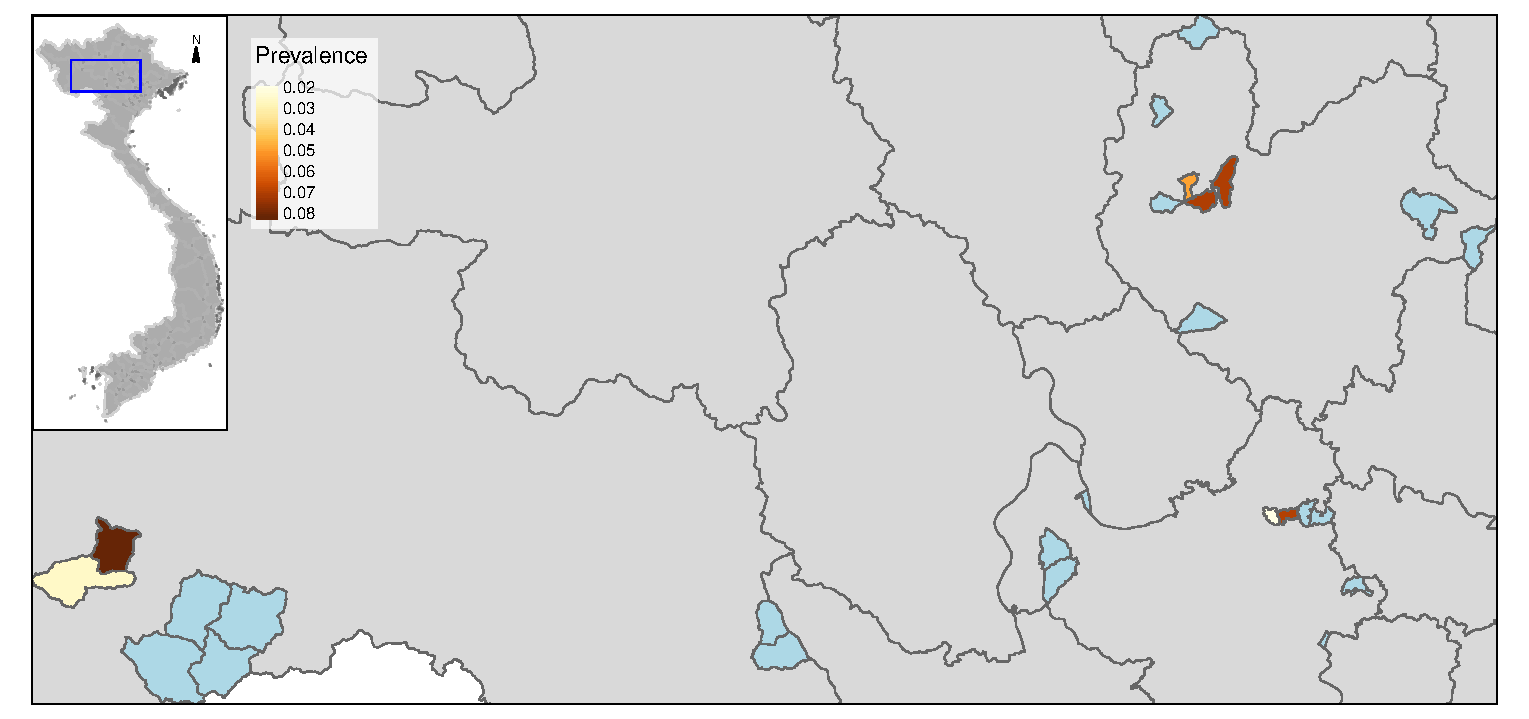
\includegraphics[width=1\textwidth]{map06_spring.pdf}
\end{center}
\end{frame}

% \begin{frame}
% \vspace{-0.6cm}
% \begin{columns}[t]
% \begin{column}{7cm}
% \begin{center}
% \includegraphics[width=1\textwidth]{figs/SI.png}\\
% Ignaz Philipp Semmelweis (1818--1865)\\
% \url{https://semmelweismuseum.hu/}\\
% {\small\url{https://www.facebook.com/SOMuseum}}
% \end{center}
% \end{column}
% \begin{column}{5cm}
% \begin{itemize}
%  \item 1847: chlorinated lime for hand washing
%  \item 1879: Pasteur presented \textit{streptococcus} from childbed fever
%  \item causality? association? efficiency
% \end{itemize}
% \vspace{1cm}
% \textit{Leviticus 13,4}:\\
% {\scriptsize%
% \textit{''If the shiny spot on the skin is white but does not appear to be more than skin deep and the hair in it has
% not turned white, the priest is to isolate the affected person for seven days.''}}
% \end{column}
% \end{columns}
% \end{frame}
